\documentclass{fkpresentation}

% \setcounter{errorcontextlines}{999}
% Information to be included in the title page:
\title{\textmd{The Euler-Lagrange Equation}}
\author{Forest Kobayashi}
\institute{Harvey Mudd College}
\date{April 1st, 2018}

\usepackage{fkmath}
\usepackage{animate}
\usetikzlibrary{external}
% \tikzexternalize

\begin{document}
\frame{\titlepage}
\section{Motivating Problems}



% \begin{frame}{Airline}
%   \begin{figure}[h]
%     \centering
%     \animategraphics[keepaspectratio,height=6cm]{20}{animations/straight/straight-}{0}{128}
%   \end{figure}
% \end{frame}

\begin{frame}{Wind}
  \begin{figure}[h]
    \centering
    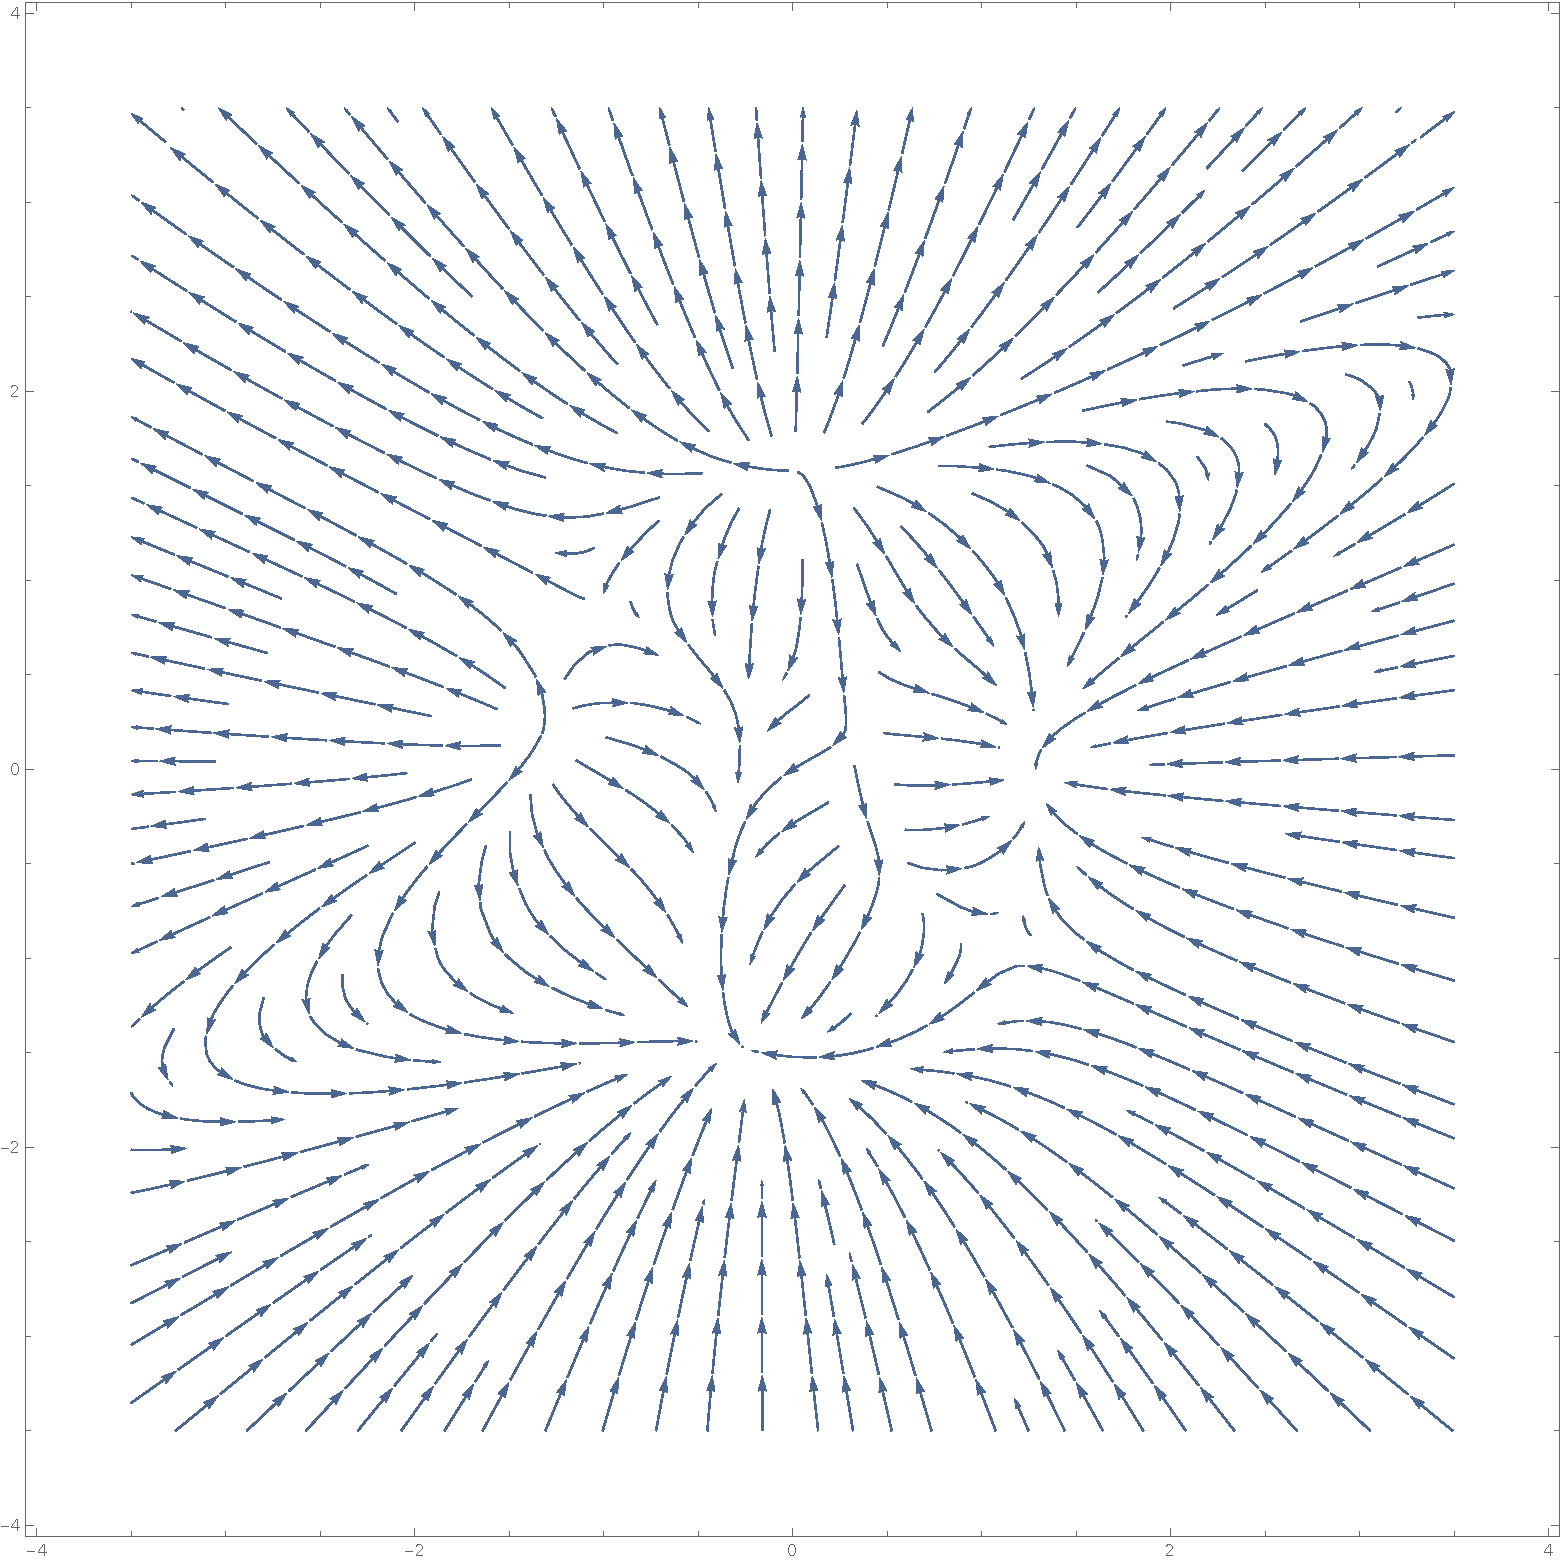
\includegraphics[keepaspectratio,height=5cm]{vector-field.pdf}
    \caption{Wind Vector Field}
    \label{fig:wind}
  \end{figure}
\end{frame}

\begin{frame}{Underlying Scalar Function}
  \begin{figure}[h]
    \centering
    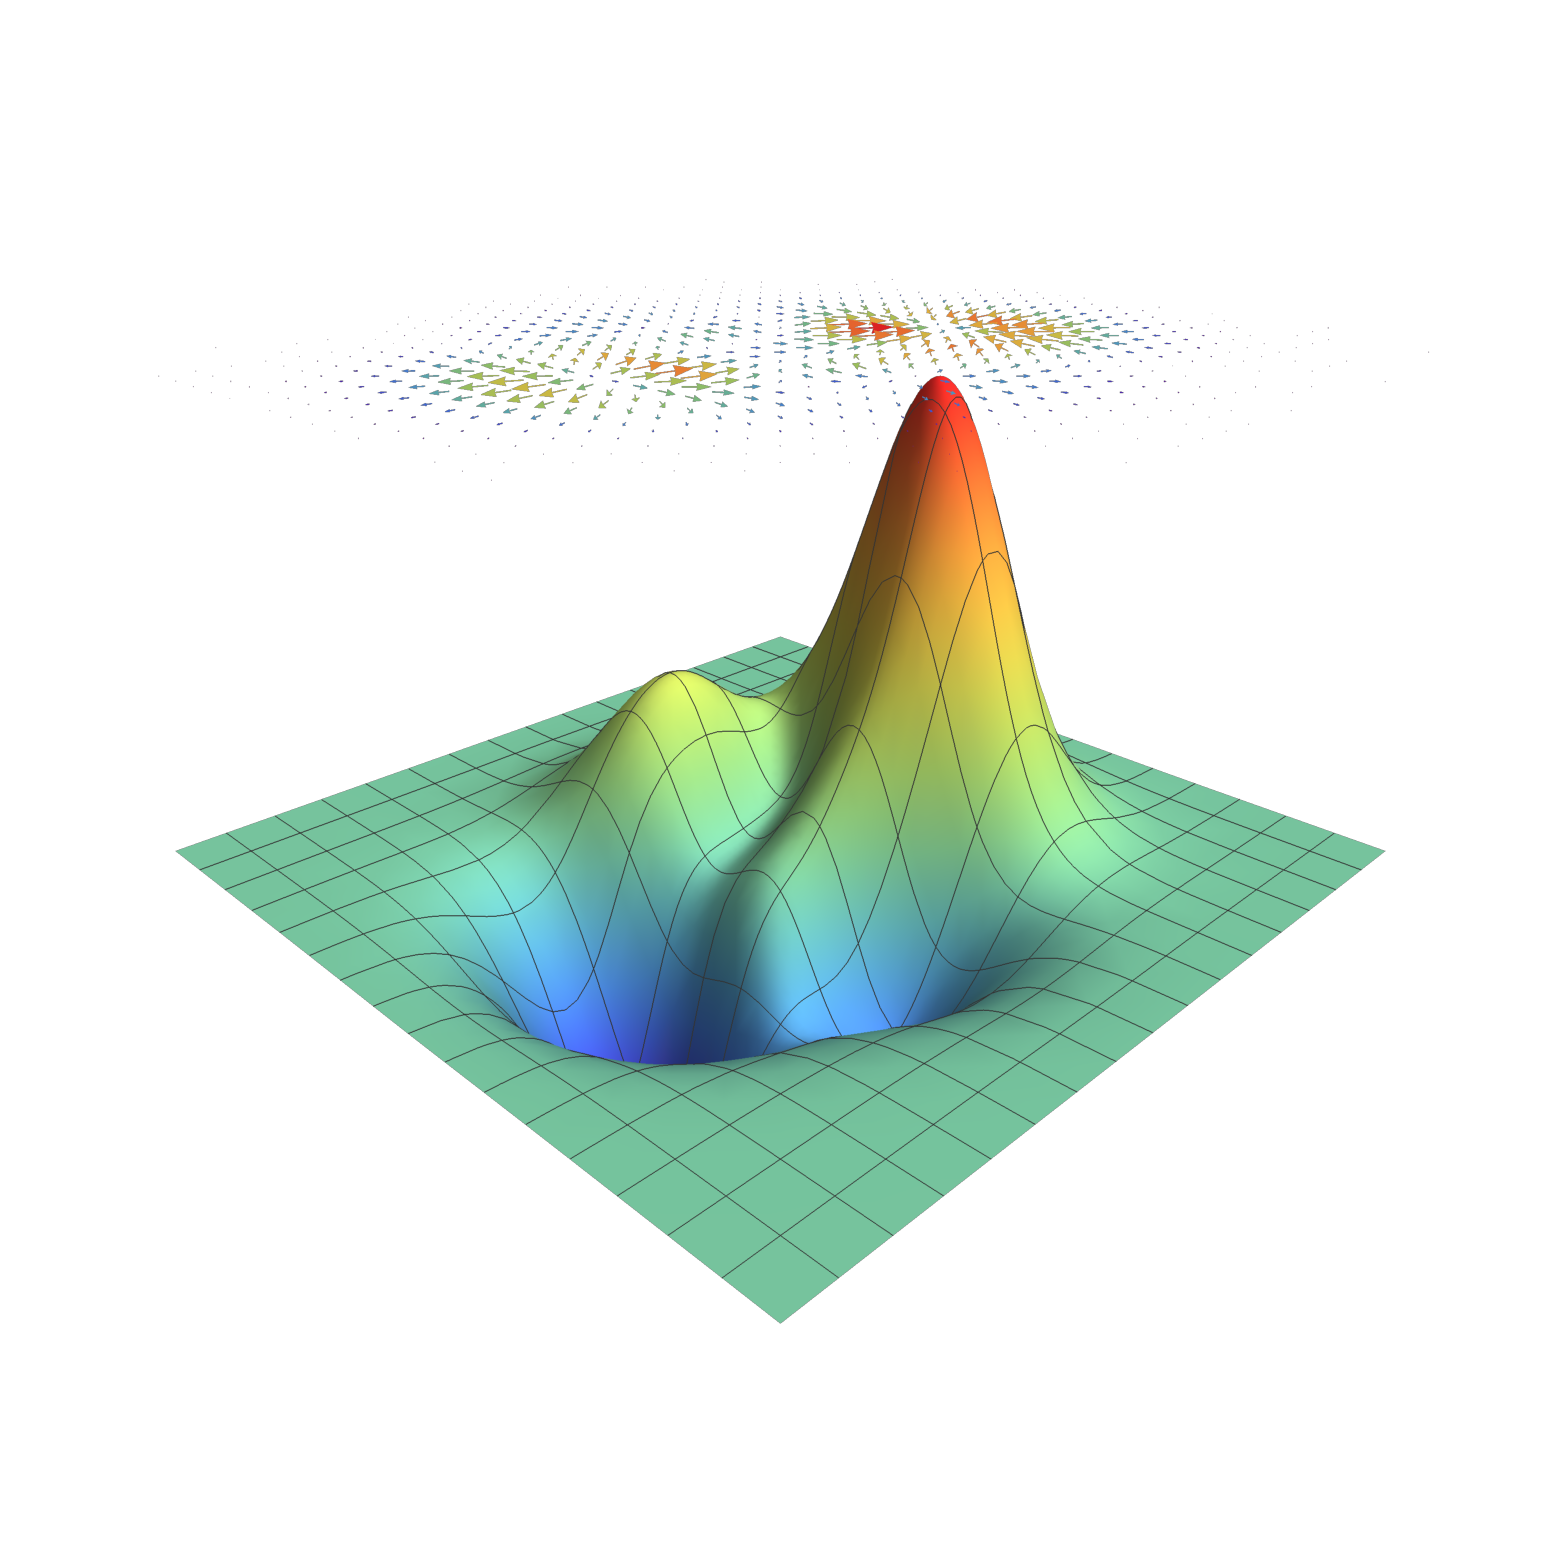
\includegraphics[keepaspectratio,height=7cm]{vect-to-scalar.pdf}
  \end{figure}
\end{frame}

% \begin{frame}{Shortest Time Path}
%   \vfill
%   \begin{figure}[h]
%     \begin{tikzpicture}[scale=2]
%       \def\r{1} % radius
%       \def\c{1.4} % center
%       \coordinate (O) at (0,0);
%       \coordinate (A) at (0,2*\r);
%       \coordinate (B) at (pi, 0);

%       % Cycloid
%       \draw[red,domain=0:pi,samples=50] plot ({\x - sin(\x r)},{\r+cos(\x r)});

%       % Straight line
%       \draw[blue] (A) -- (B);

%       % The other two
%       \draw[green, domain=0:pi, samples=50] plot ({\x}, {(-2/pi)*(\x-pi)*exp(-4*\x)});
%       \draw[orange, domain=0:pi, samples=50] plot ({\x}, {(-2/pi)*(\x-pi)*exp(\x/3)});

%       % Release point
%       \draw[fill=black] (A) circle (.75pt);

%       % End point
%       \draw[fill=black] (B) circle (.75pt);

%     \end{tikzpicture}
%   \end{figure}
%   \vfill
% \end{frame}


\begin{frame}{Shortest Path}
  \begin{figure}[h]
    \vfill
    \centering
    \begin{tikzpicture}[
      scale=1.5,
      declare function = {
        a(\x, \y) = 3*(1-\x)^2 * exp(-(\x^2)-(\y+1)^2);
        b(\x, \y) = -10*(\x/5 - \x^3 + \y^5) * exp(-\x^2 - \y^2);
        c(\x, \y) = -exp(-(\x+1)^2 - \y^2)/3;
        Z(\x, \y) = a(\x,\y) + b(\x,\y) + c(\x,\y);
        paraX(\t) = (0 <= \t, \t < 0.224045) * (1.11203 + \t * (-3.31095 + (-2.01459 - 0.455886 * \t) * \t)) +
        and(0.224045 <= \t, \t < 0.334761) * (1.01126 + \t * (-1.96156 + \t * (-8.03743 + 8.50486 * \t)))  +
        and(0.334761 <= \t, \t < 0.445505) * (1.32733 + \t * (-4.79407 + (0.423885 + 0.079617 * \t) * \t)) +
        and(0.445505 <= \t, \t < 0.555932) * (1.33869 + \t * (-4.8706 + (0.595662 - 0.0489086 * \t) * \t)) +
        and(0.555932  = \t)                * (-1.19334)                                              +
        and(0.555932  < \t, \t < 0.667191) * (0.69873 + \t * (-1.41713 + \t * (-5.61637 + 3.67579 * \t)))  +
        and(0.667191  = \t)                * (-1.65517)                                              +
        and(0.667191  < \t, \t < 0.778976) * (4.39251 + \t * (-18.0261 + (19.2775 - 8.76134 * \t) * \t))   +
        and(0.778976  = \t)                * (-2.0931)                                               +
        and(0.778976  < \t, \t <= 1.)      * (1.32733 + \t * (-4.79407 + (0.423885 + 0.079617 * \t) * \t));
      }
      ]
      \begin{axis}[
        view={230}{40},
        % axis lines=center,
        % enlargelimits,
        hide x axis,
        hide y axis,
        hide z axis,
        % tick align=inside,
        domain=-3.5:3.5,
        samples=10,
        % grid=major,
        % minor tick num=5
        ]
        \addplot3 [surf] {Z(x,y)};
        \addplot3 [only marks, mark options={scale=.3}] table[row sep=crcr] {
          x y z \\
          1.5 1.7 -.652 \\
          -3 -.3 4.563 \\
        };
        \addplot3[variable=t, domain=0:1] (paraX(t), 0, 0);
      \end{axis}
    \end{tikzpicture}
    \vfill
  \end{figure}
\end{frame}

% Function:
% z = 3 * (1-x)^2 * exp(-(x^2) - (y+1)^2) - 10 * (x/5 - x^3 - y^5) * exp(-x^2 -
% y^2) - 1/3 * exp(-(x+1)^2 - y^2)



\begin{frame}{The statement}
  \begin{theorem}[Euler-Lagrange]
    Let $\Qq(t) : \RR \to \RR^n$ be a path. Then if $\Qq(t)$ is an
    extreme value of the functional
    \[
      S(\Qq) = \int_a^b \mc L\pn{t, \Qq(t), \dot{\Qq}(t)} \dd t
    \]
    then $\Qq$ is a solution to the differential equation
    \[
      \pd{\mc L}{\Qq} - \od{}{t} \pn{\pd{\mc L}{\dot{\Qq}}} = 0
    \]
  \end{theorem}
\end{frame}

\section{Proof Sketch}

\begin{frame}
  \begin{figure}[h]
    \centering
    \begin{tikzpicture}
      \pgfmathsetmacro{\xmin}{-.2};
      \pgfmathsetmacro{\ymin}{-.2};
      \pgfmathsetmacro{\xmax}{6};
      \pgfmathsetmacro{\ymax}{5};

      \pgfmathsetmacro{\extraforaxes}{.2};

      \pgfmathsetmacro{\epsilon}{.1};

      \draw[->] (\xmin,0) -- (\xmax+\extraforaxes, 0) node[below] {$x$};
      \draw[->] (0,\ymin) -- (0, \ymax+\extraforaxes) node[left] {$y$};

      \draw[domain=1.5:5.5, smooth, variable=\x, blue] plot ({\x-.5},
      {-1.7 + \x * (3.31667 + (-0.9 + 0.0833333 * \x) * \x)});

      \node[
      circle,
      draw=black,
      fill=white,
      inner sep=0pt,
      minimum size=5pt
      ] (y0) at (1, 1.56875) {};

      \node[
      circle,
      draw=black,
      fill=white,
      inner sep=0pt,
      minimum size=5pt
      ] (y1) at (5, 3.18126) {};

      % \draw[domain=\xmin:\xmax, smooth, variable=\x, blue] plot ({\x}, )

      % \draw[scale=0.5,domain=-3:3,smooth,variable=\x,blue] plot ({\x}, {\x*\x});
      % \draw[scale=0.5,domain=-3:3,smooth,variable=\y,red]  plot ({\y*\y}, {\y});
    \end{tikzpicture}
  \end{figure}
\end{frame}


% \section{Bibliography}
% \begin{frame}
%   \frametitle{References}
%   \bibliographystyle{alpha}
%   %   \bibliographystyle{IEEE}
%   \bibliography{aha.bib}
% \end{frame}

\end{document}


%%% Local Variables:
%%% TeX-master: t
%%% TeX-engine: default-shell-escape
%%% TeX-command-extra-option: -pdf
%%% End: